\documentclass[11pt]{article}

\usepackage[margin=2cm]{geometry}
\usepackage{titling}
\usepackage[T1]{fontenc}
\usepackage{tabularx}
\usepackage{amsfonts}
\usepackage{amsmath}
\usepackage{stackengine}
\usepackage{graphicx}
\usepackage{subcaption}
\usepackage{changepage}
\usepackage{algorithm}
\usepackage[noend]{algpseudocode}


\pretitle{\begin{center}\Huge\bfseries}
\posttitle{\par\end{center}\vskip 0.5em}
\preauthor{\begin{center}\Large}
\postauthor{\end{center}}
\predate{\par\large\centering}
\postdate{\par}

\title{Obliczenia naukowe - lab 4}
\author{Jakub Musiał 268442}
\date{Grudzień 2023}

\begin{document}

\maketitle

\hspace{1cm}

\section*{Zadania 1-4: Biblioteka}
    \subsection*{Problem}
        Zaimplementować bibiliotekę służącą do wizualizacji interpolacji wielomianowej.

    \subsection*{Rozwiązanie}
        Implementacja biblioteki: \texttt{interpolation.jl}
        \newline
        Program testujący: \texttt{interpolation\_test.jl}

        \subsubsection*{Zadanie 1: Ilorazy różnicowe}
        Dla danych węzłów $x_i, x_{i+1}, ..., x_j$ oraz znanych dla nich wartości funkcji $f$
        definiujemy rekurencyjnie iloraz różnicowy $f[x_i, x_{i+1}, ..., x_j]$ :
        \begin{equation}
            \left
            \lbrace
            \begin{array}{l}
                f[x_i] \gets f(x_i) \\
                f[x_i, ..., x_j] \gets \frac{f[x_{i+1}, ..., x_j] - f[x_i, ..., x_{j-1}]}{x_j - x_i}
            \end{array}
            \right.
        \end{equation}

        \noindent Dla tak zdefiniowanych ilorazów różnicowych funckja powinna zwracać wektor zawierający ilorazy
        różnicowe $f[x_0], ..., f[x_0, ..., x_n]$ na podstawie zadanych węzłów $x = (x_0, ..., x_n)$ oraz wartości funkcji
        $f$ w tych węzłach.

        \noindent Algorytm wyznaczający wektor ilorazów różnicowych opiera się na opisanym powyżej wzorze rekurencyjnym.
        Żeby jednak uniknąć używania tablicy 2-wymiarowej możemy go zmodyfikować tak, żeby odpowiednio aktualizować
        wartości ilorazów różnicowych na podstawie wartości wyliczonych w poprzednich iteracjach. Wiemy, że
        $f[x_0] = f(x_0)$, więc możemy pominąć wyliczanie tej wartości. Pozostałe wartości aktualizujemy, licząc kolejne
        wartości $f[x_i, ..., x_j]$ wg. schematu:

        \newcommand{\rotatedarrow}{\rotatebox[origin=c]{-30}{$\rightarrow$}}
        \newcommand{\rotateddots}{\rotatebox[origin=c]{45}{$\vdots$}}

        \begin{center}
        \begin{math}
            \begin{array}{cccccccc}
                f[x_0] \\
                & \rotatedarrow \\
                f[x_1] & \rightarrow & f[x_0, x_1] \\
                & \rotatedarrow & & \rotatedarrow \\
                f[x_2] & \rightarrow & f[x_1, x_2] & \rightarrow & f[x_0, x_1, x_2] \\
                \vdots & \rotateddots & \vdots & \rotateddots & \vdots & \rotateddots \\
                f[x_n] & \rightarrow & f[x_{n-1}, x_n] & \rightarrow & \hdots & \rightarrow & f[x_0, ..., x_n]
            \end{array}
        \end{math}
        \end{center}

        \newpage

        \begin{algorithm}[h!]
        \caption{Ilorazy różnicowe}\label{alg:differential_quotients}
        \begin{algorithmic}[1]
            \Require $x, f$
            \State $n \gets length(x)$
            \State $\text{fx} \gets f$
            \For{$i \gets 2$ to $n$}
                \Comment $f[x_0] = f(x_0)$ : wykonane podczas kopiowania (linia \texttt{2})
                \For{$j \gets n-1$ down to $1$}
                    \State $\text{fx}[j] = (\text{fx}[j] - \text{fx}[j-1]) / (x[j] - x[j-i+1])$
                \EndFor
            \EndFor
            \State \Return fx
        \end{algorithmic}
        \end{algorithm}

        \noindent \newline

        \subsubsection*{Zadanie 2: Wartość wielomianu interpolacyjnego w postaci Newtona}
        Funkcja powinna obliczać wartość wielomianu interpolacyjnego w postaci Newtona w czasie liniowym dla zadanej
        zadanego wektora węzłów $x = (x_0, ..., x_n)$ oraz wektora ilorazów różnicowych
        $\text{fx} = (f[x_0], ..., f[x_0, ... x_n])$ w punkcie $t$.

        \noindent Wartość wielomianu w postaci Newtona w punkcie $t$ jest równa
        $N_n(t) = \sum_{i = 0}^{n}(q_i \cdot \prod_{j = 0}^{i - 1}(t - x_i))$, gdzie $q_i = f[x_0, ..., x_i]$.
        Zatem aby ją wyznaczyć możemy wykorzystać uogólniony schemat Hornera:
        \[ w_n(x) = q_n \]
        \[ w_i(x) = q_i + (x - x_i) + w_{i+1}(x) \]
        Skąd otrzymujemy oczekiwany wynik $N_n(t) = w_0(t)$.

        \begin{algorithm}[h!]
        \caption{Wartość w postaci Newtona}\label{alg:newton_value}
        \begin{algorithmic}[1]
            \Require $x, \text{fx}, t$
            \State $n \gets length(x)$
            \State $\text{nt} \gets \text{fx}[n]$
            \For{$i \gets n-1$ down to $1$}
                \State $\text{nt} \gets \text{fx}[i] + (t - x[i]) * \text{nt}$
            \EndFor
            \State \Return nt
        \end{algorithmic}
        \end{algorithm}

        \noindent \newline

        \subsubsection*{Zadanie 3: Postać naturalna wielomianu}
        Na podstawie zadanego wektora węzłów $x = (x_0, ..., x_n)$ oraz wektora ilorazów różnicowych
        $\text{fx} = (f[x_0], ..., f[x_0, ... x_n])$ funkcja powinna w czasie kwadratowym zwracać wektor
        $a = (a_0, ..., a_n)$ współczynników wielomianiu w postaci naturalnej:
        \begin{center}
        \begin{math}
            w(x) = \sum_{i = 0}^{n}a_i \cdot x^i
        \end{math}
        \end{center}

        \noindent Wiedząc, że $a_n = f[x_0, ..., x_n]$, możemy wyznaczyć wektor współczynników $a$, wykonując przejścia
        odwrotne do tych w schemacie Hornera i tym samym wyznaczając w i-tej iteracji współczynnik przy wyrazie $x^i$.

        \begin{algorithm}[h!]
        \caption{Postać naturalna}\label{alg:natural_coefficients}
        \begin{algorithmic}[1]
            \Require $x, \text{fx}$
            \State $n \gets length(x)$
            \State $a \gets zeros(n)$
            \For{$i \gets n-1$ down to $1$}
                \State $a[i] \gets \text{fx}[i] - x[i] \cdot a[i+1]$
                \For{$j \gets i+1$ to $n-1$}
                    \State $a[j] \gets a[j] - x[i] \cdot a[j+1]$
                \EndFor
            \EndFor
            \State \Return $a$
        \end{algorithmic}
        \end{algorithm}

        \newpage
        \noindent \newline

        \subsubsection*{Zadanie 4: Wizualizacja interpolacji}
        Funkcja powinna zinterpolować zadaną funkcję $f$ wielomianem stopnia $n$ na podstawie węzłów z przedziału
        $[a, b]$ oraz wykonać wykres funkcji $f$, jak i jej wielomianu interpolacyjnego w zadanym przedziale.
        \newline
        Funkcja najpierw wyznacza wektor $x = (x_0, ..., x_n)$ (równo rozmieszczone węzły w przedziale $[a, b]$)
        oraz dla węzłów $x$ wyznacza wektor ilorazów różnicowych $\text{fx} = (f[x_0], ..., f[x_0, ... x_n])$.
        Następnie dla pewnej liczby $n_{plot}$ (ponownie równo rozmieszczonych w przedziale $[a, b]$) punktów rysowanych
        na wykresie wyznacza wartości funkcji $f$ oraz wartości wielomianu interpolacyjnego, wykorzystując funkcję z
        zadania \textit{3}.

    \noindent \newline

\section*{Zadanie 5}
    \subsection*{Problem}
        Wywołać funkcją wizualizującą interpolację funkcji dla zadanych przykładów:
        \begin{itemize}
            \item $f(x) = e^x \land [a, b] = [0, 1]$
            \item $f(x) = x^2 \cdot \sin{x} \land [a, b] = [-1, 1]$
        \end{itemize}
        Oraz dla stopni wielomianów interpolacyjnych $n \in \{5, 10, 15\}$.

    \subsection*{Rozwiązanie}
        Plik źródłowy: \texttt{ex5.jl}

    \subsection*{Wyniki i obserwacje}
        Na podstawie wygenerowanych wykresów możemy zauważyć, że obie badane funkcje na zadanych przedziałach są bardzo
        dobrze przybliżone za pomocą interpolacji wielomianowej. Dla wszystkich badanych stopni wielomianu interpolacyjnego
        otrzymane aproksymacje niemal się pokrywają z odpowiadającymi im funkcjami.

        \begin{figure}[htbp]
        \centering
            \begin{subfigure}[b]{0.45\textwidth}
                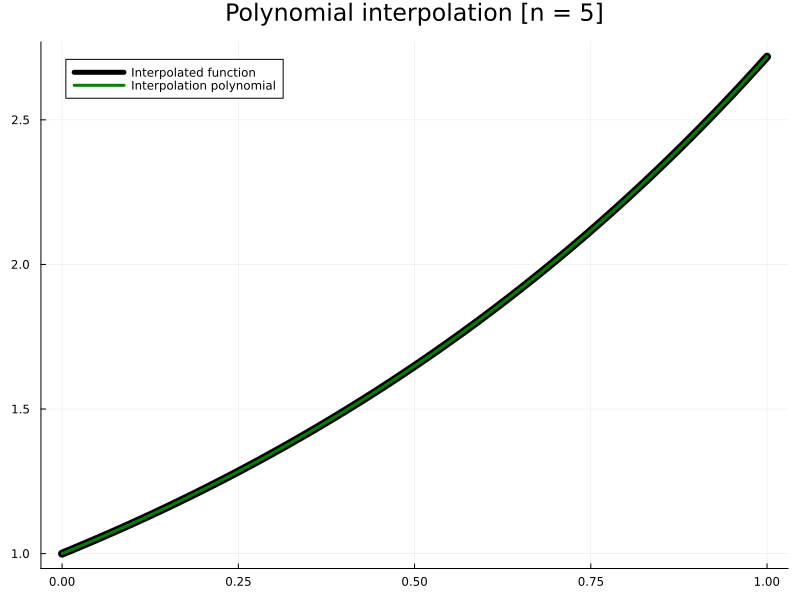
\includegraphics[width=\linewidth]{img/ex5_f1_n5.png}
            \end{subfigure}
            \hfill
            \begin{subfigure}[b]{0.45\textwidth}
                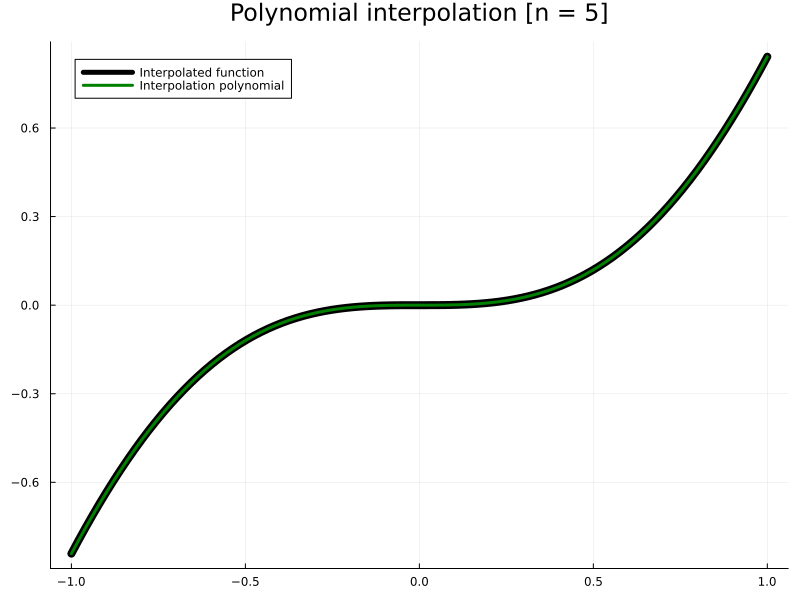
\includegraphics[width=\linewidth]{img/ex5_f2_n5.png}
            \end{subfigure}
            \begin{subfigure}[b]{0.45\textwidth}
                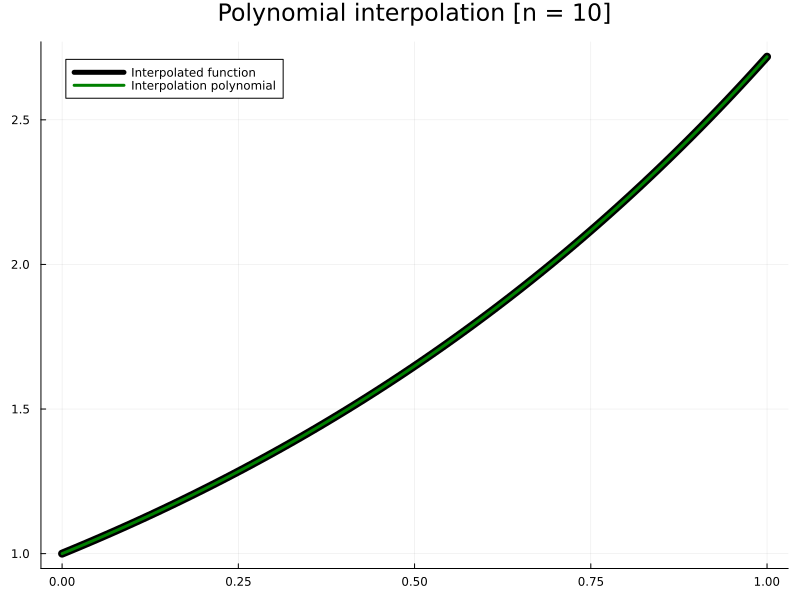
\includegraphics[width=\linewidth]{img/ex5_f1_n10.png}
            \end{subfigure}
            \hfill
            \begin{subfigure}[b]{0.45\textwidth}
                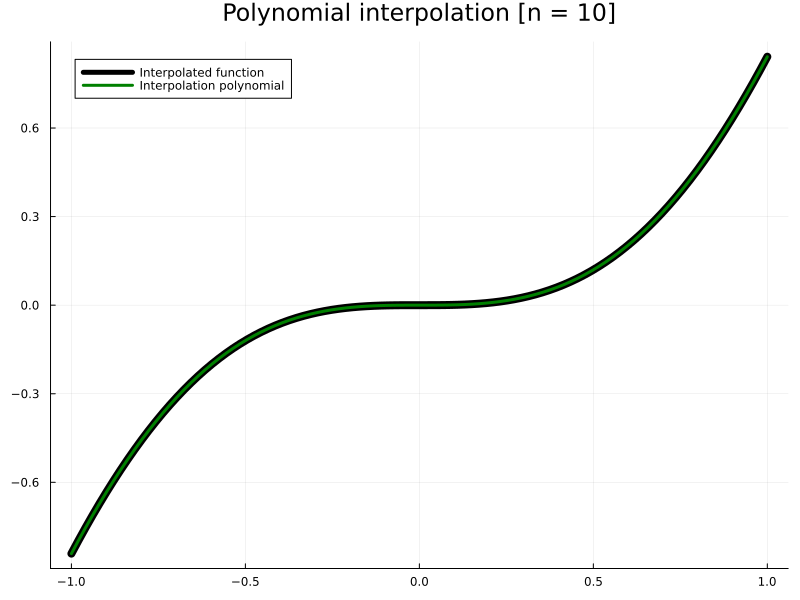
\includegraphics[width=\linewidth]{img/ex5_f2_n10.png}
            \end{subfigure}
            \begin{subfigure}[b]{0.45\textwidth}
                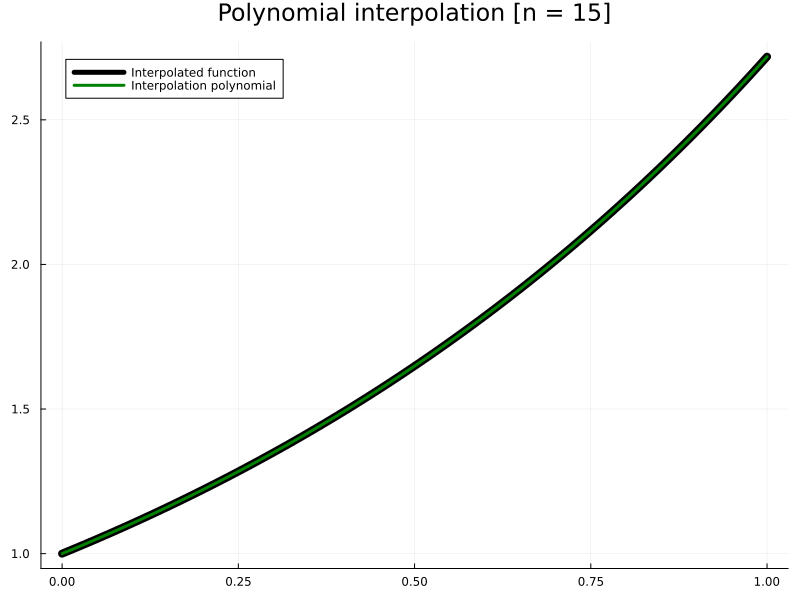
\includegraphics[width=\linewidth]{img/ex5_f1_n15.png}
                \caption{Interpolacja funckji $f(x) = e^x$ w przedziale $[0, 1]$}
            \end{subfigure}
            \hfill
            \begin{subfigure}[b]{0.45\textwidth}
                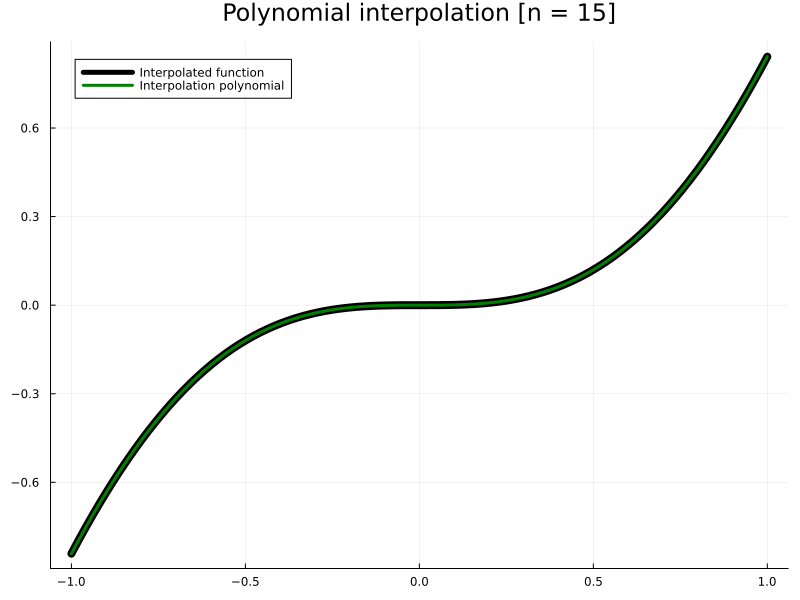
\includegraphics[width=\linewidth]{img/ex5_f2_n15.png}
                \caption{Interpolacja funckji $f(x) = x^2 \cdot \sin{x}$ w przedziale $[-1, 1]$}
            \end{subfigure}
            \caption{Wizualizacja interpolacji funckji z zadania 5}
        \end{figure}

    \newpage

\section*{Zadanie 6}
    \subsection*{Problem}
        Wywołać funkcją wizualizującą interpolację funkcji dla zadanych przykładów:
        \begin{itemize}
            \item $f(x) = |x| \land [a, b] = [-1, 1]$
            \item $f(x) = \frac{1}{1 + x^2} \land [a, b] = [-5, 5]$
        \end{itemize}
        Oraz dla stopni wielomianów interpolacyjnych $n \in \{5, 10, 15\}$.

    \subsection*{Rozwiązanie}
        Plik źródłowy: \texttt{ex6.jl}

    \subsection*{Wyniki i obserwacje}
        Zauważmy, że funckje badane w tym zadaniu nie dają się tak dobrze interpolować, jak poprzednie przykłady.
        Występuje tutaj efekt Runge'go, który polega na pogarszaniu jakości interpolacji mimo zwiększania stopnia $n$
        wielomianu interpolacyjnego. Pogarszanie to jest szczególnie zauważalne na krańcach zadanego przedziału, na
        którym funkcja jest interpolowana. Jest to skutek założenia stałej odległości między węzłami. Sposoben na
        zniwelowanie tego efektu może być zagęszczanie węzłów na końcach przedziałów interpolacji.
        \newline
        Dodatkowo efekt ten może występować w sytuacjach, kiedy funkcja odbiega od funkcji gładkiej, jak jest w
        pierwszej z badanych w tym zadaniu funkcji - $f(x) = |x|$, która nie jest różniczkowalna, więc tym bardziej
        nie może być gładka.

        \noindent\newline

        \begin{figure}[htbp]
        \centering
            \begin{subfigure}[b]{0.45\textwidth}
                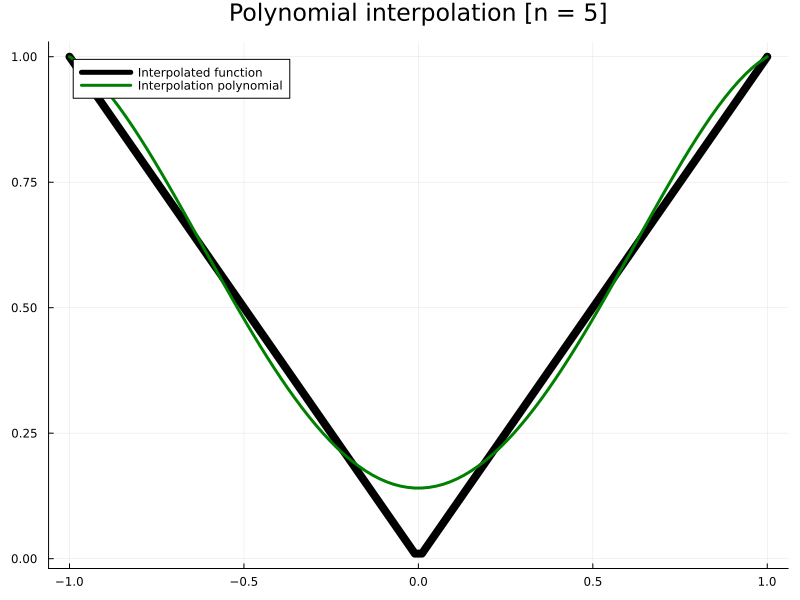
\includegraphics[width=\linewidth]{img/ex6_f1_n5.png}
            \end{subfigure}
            \hfill
            \begin{subfigure}[b]{0.45\textwidth}
                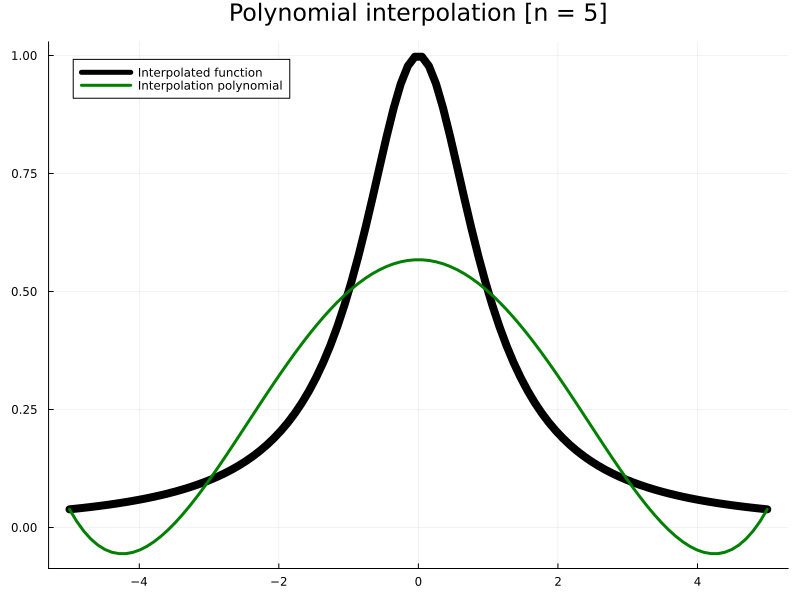
\includegraphics[width=\linewidth]{img/ex6_f2_n5.png}
            \end{subfigure}
        \end{figure}
        \newpage
        \begin{figure}[htbp]
            \begin{subfigure}[b]{0.45\textwidth}
                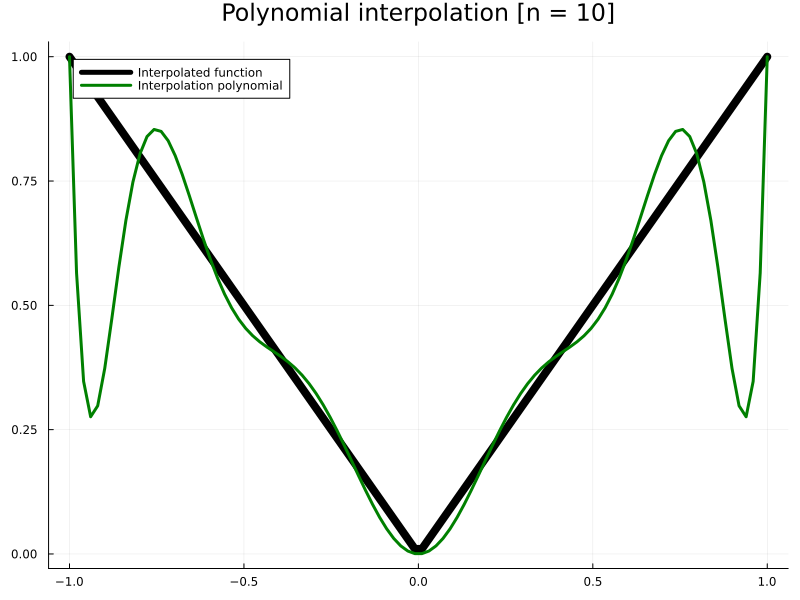
\includegraphics[width=\linewidth]{img/ex6_f1_n10.png}
            \end{subfigure}
            \hfill
            \begin{subfigure}[b]{0.45\textwidth}
                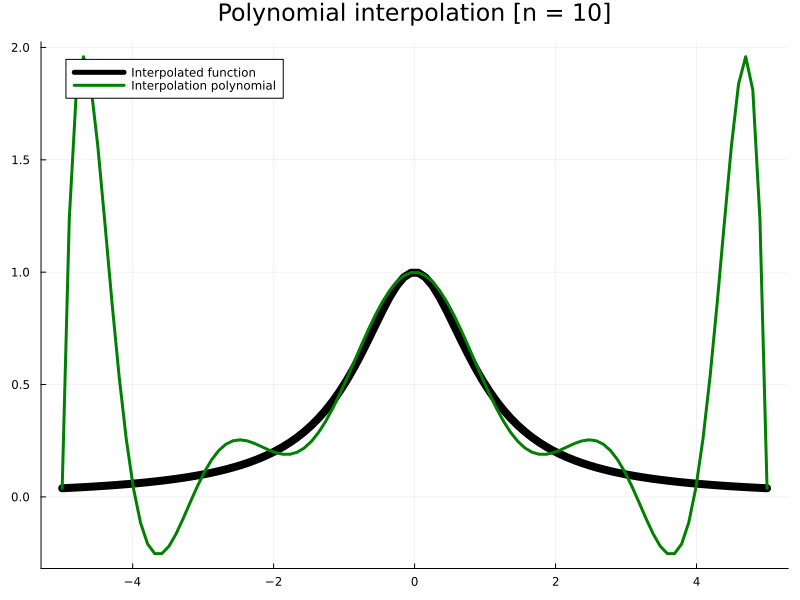
\includegraphics[width=\linewidth]{img/ex6_f2_n10.png}
            \end{subfigure}
            \begin{subfigure}[b]{0.45\textwidth}
                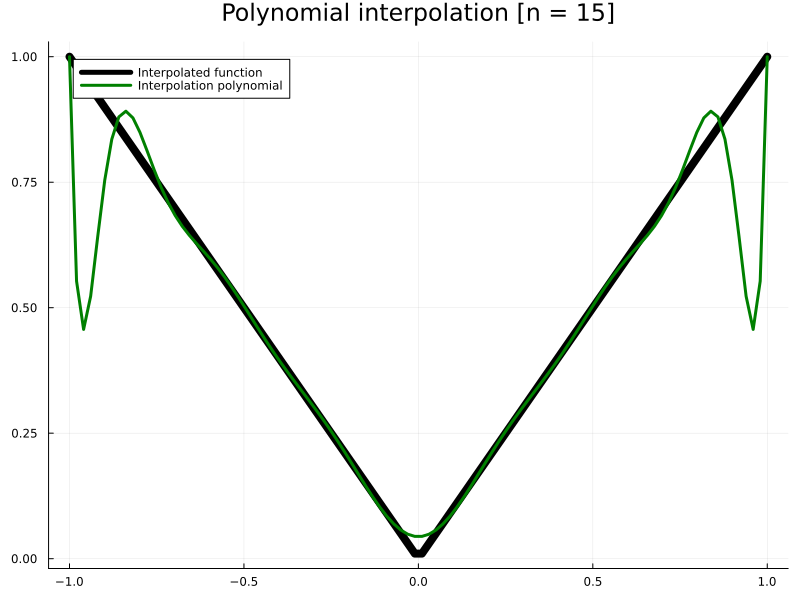
\includegraphics[width=\linewidth]{img/ex6_f1_n15.png}
                \caption{Interpolacja funckji $f(x) = |x|$}
            \end{subfigure}
            \hfill
            \begin{subfigure}[b]{0.45\textwidth}
                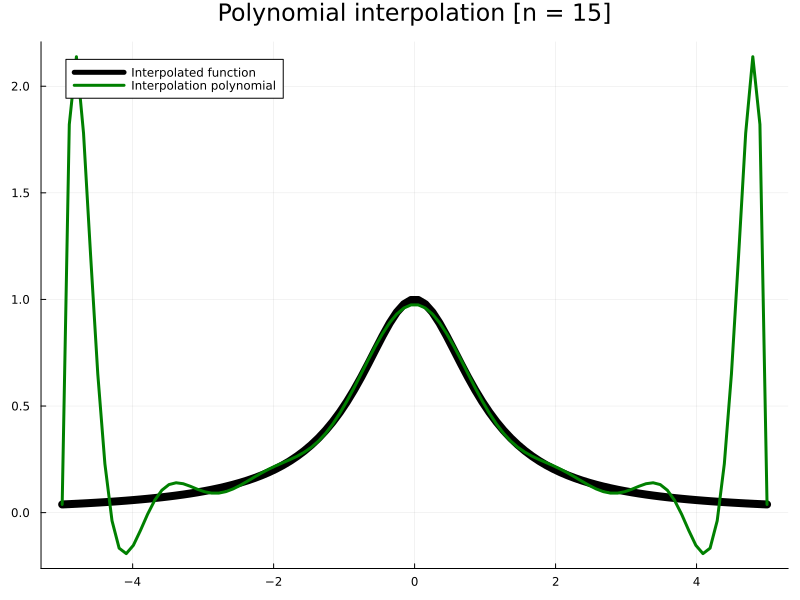
\includegraphics[width=\linewidth]{img/ex6_f2_n15.png}
                \caption{Interpolacja funckji $f(x) = \frac{1}{1 + x^2}$}
            \end{subfigure}
            \caption{Wizualizacja interpolacji funckji z zadania 6}
        \end{figure}


\end{document}
